\label{sec:intro-contexte}

L'évolution des technologies du web a conduit à l'avènement de ce qui est communément appelé le Web 2.0.
La principale caractéristique de ce média est la possibilité aux utilisateur-rices non plus seulement de le consulter, mais aussi d'y contribuer.

Ces nouvelles fonctionnalités ont permis l'apparition d'applications incitant les utilisateur-rices à créer et partager leur propre contenu, ainsi que d'échanger avec d'autres utilisateur-rices à ce sujet.
Un cas particulier de ces applications proposent aux utilisateur-rices de travailler ensemble pour la création d'un même contenu, en d'autres termes de collaborer.
Nous appelons ces applications des \emph{systèmes collaboratifs} :
\begin{definition}[Système collaboratif]
  \label{def:collaborative-system}
  Un système collaboratif est un système supportant ses utilisateur-rices dans leurs processus de collaboration pour la réalisation de tâches.
\end{definition}

De nos jours, ces systèmes font parties des applications les plus populaires du paysage internet, \eg la suite logicielle dont fait partie GoogleDocs compte 2 milliards d'utilisateur-rices \cite{2020-google-g-suite-users}, Wikipedia 788 millions \cite{2022-09-monthly-active-users-wikipedia}, Quora 300 millions \cite{2022-01-monthly-active-users-social-networks} ou encore GitHub 60 millions \cite{2022-github-users}.
De leur côté, d'autres plateformes fédèrent leur communautés en organisant ponctuellement des collaborations éphémères et généralement massives, \eg r/Place \cite{2022-rplace} ou TwitchPlaysPokemon \cite{2014-twitch-plays-pokemon}.\\

En raison de leur popularité, les systèmes collaboratifs doivent assurer plusieurs propriétés pour garantir leur bon fonctionnement et qualité de service : une haute disponibilité, tolérance aux pannes et capacité de passage à l'échelle.
\begin{definition}[Disponibilité]
  \label{def:availability}
  La disponibilité d'un système indique sa capacité à répondre à tout moment à une requête d'un-e utilisateur-rice.
\end{definition}
\begin{definition}[Tolérance aux pannes]
  La tolérance aux pannes d'un système indique sa capacité à continuer à répondre aux requêtes malgré l'absence de réponse d'un ou plusieurs de ses composants.
\end{definition}
\begin{definition}[Capacité de passage à l'échelle]
  La capacité de passage à l'échelle d'un système indique sa capacité à traiter un volume toujours plus conséquent de requêtes.
\end{definition}

Pour cela, ces systèmes adoptent une architecture décentralisée, que nous illustrons par la \autoref{fig:decentralised-system}.
\begin{figure}[!ht]
  \centering
  \resizebox{0.3 \columnwidth}{!}{
    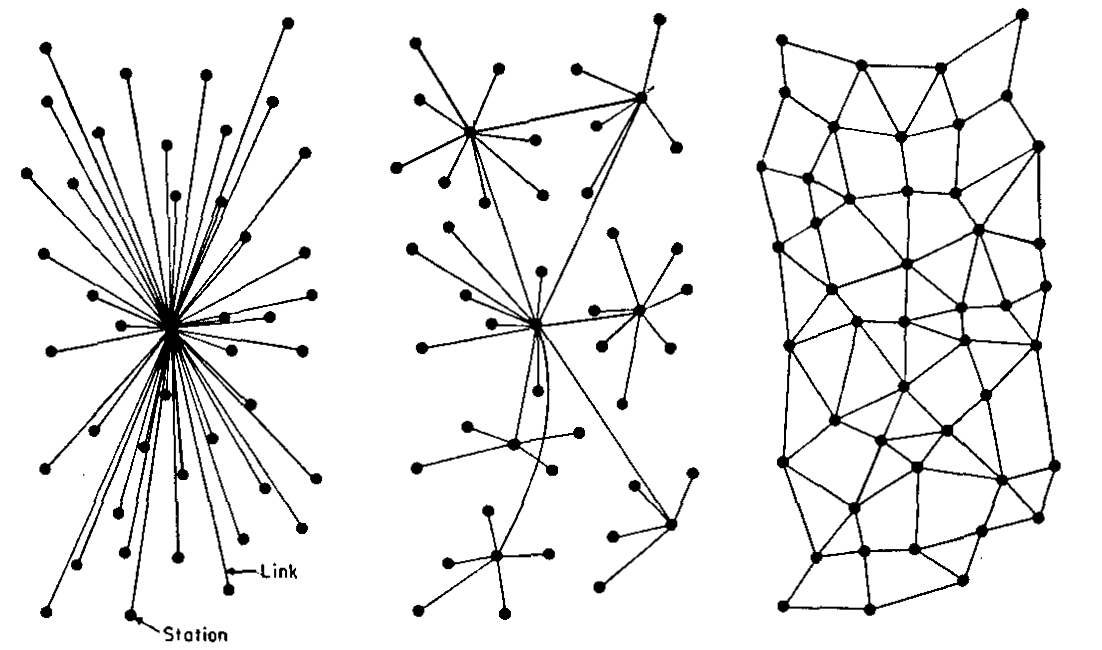
\includegraphics[trim=12cm 0cm 13cm 0cm, clip]{img/centralised-decentralised-distributed}
  }
  \caption[Caption for decentralised-system]{
    Représentation d'une architecture décentralisée \cite{1964-distributed-communications-networks-baran}.
    Les noeuds aux extrêmités du graphe correspondent à des clients, les noeuds internes à des serveurs et les arêtes du graphe représentent les connexions entre appareils.
  }
  \label{fig:decentralised-system}
\end{figure}

Dans ce type d'architecture, les responsabilités, tâches et la charge travail sont réparties entre un ensemble de serveurs.
Malgré ce que le nom de cette architecture peut suggérer, il convient de noter que les serveurs jouent toujours un rôle central dans ces systèmes,.
En effet, ces systèmes reposent toujours sur leurs serveurs pour authentifier les utilisateur-rices, stocker les données de leurs utilisateur-rices ou encore fusionner les modifications effectuées par ces dernier-es.\\
% La nuance porte seulement sur le fait que ce n'est plus un serveur unique qui est en charge de ces tâches, mais un ensemble de serveurs.

Bien que cette architecture système permette de répondre aux problèmes d'ordre technique que nous présentons précédemment, elle souffre néanmoins de limites.
Notamment, de part le rôle prédominant que jouent les serveurs dans les systèmes décentralisés, ces derniers échouent à assurer un second ensemble de propriétés que nous jugeons néanmoins fondamentales :
\begin{definition}[Confidentialité des données]
  \label{def:confidentialite}
  La confidentialité des données d'un système indique sa capacité à garantir à ses utilisateur-rices que leurs données ne seront pas accessibles par des tiers non autorisés ou par le système lui-même.
\end{definition}
\begin{definition}[Souveraineté des données]
  \label{def:souverainete}
  La souveraineté des données d'un système indique sa capacité à garantir à ses utilisateur-rices leur maîtrise de leurs données, \ie leur capacité à les consulter, modifier, partager, exporter; supprimer ou encore à décider de l'usage qui en est fait.
\end{definition}
\begin{definition}[Pérennité]
  \label{def:perennite}
  La pérennité d'un système indique sa capacité à garantir à ses utilisateur-rices son fonctionnement continu dans le temps.
\end{definition}
\begin{definition}[Résistance à la censure]
  \label{def:censorship}
  La résistance à la censure d'un système indique sa capacité à garantir à ses utilisateur-rices son fonctionnement malgré des actions de contrôle de l'information par des autorités.
\end{definition}

De plus, les serveurs ne sont pas une ressource libre.
En effet, ils sont déployés et maintenus par la ou les organisations qui proposent le système collaboratif.
Ces organisations font alors office d'\emph{autorités centrales} du système, \eg en se portant garantes de l'identité des utilisateur-rices, de l'authenticité d'un contenu ou encore de la disponibilité dudit contenu.

De part le fait que les autorités centrales possèdent les serveurs hébergeant le système, elles ont tout pouvoir sur ces derniers.
Ainsi, les utilisateur-rices de systèmes collaboratifs prennent, de manière consciente ou non, le risque que les propriétés présentées précédemment soient transgressées par les autorités auxquelles appartiennent ces applications ou par des tiers avec lesquelles ces autorités interagissent, \eg des gouvernements.
Plusieurs faits d'actualités nous ont malheureusement montré de tels faits, \eg la censure de Wikipedia par des gouvernements \cite{2022-wikipedia-censorship}, la fermeture de services par les entreprises les proposant \cite{2022-killed-by-google} ou encore la mise à disposition des données hébergées par des applications aux services de renseignement de différentes nations \cite{prism-guardian,prism-washington-post}.
Cependant, le coût conséquent de l'infrastructure nécessaire pour déployer des systèmes à large échelle équivalents entrave la mise en place d'alternatives, plus respectueuses de leurs utilisateur-rices.\\

\emph{Ainsi, il nous paraît fondamental de proposer des moyens technologiques rendant accessible la conception et le déploiement des systèmes collaboratifs alternatifs.
Ces derniers devraient minimiser le rôle des autorités centrales, voire l'éliminer, de façon à protéger et privilégier les intérêts de leurs utilisateur-rices.}\\

Dans cette optique, une piste de recherche que nous jugeons intéressante est celle des systèmes collaboratifs \acf{P2P}.
Cette architecture système, que nous illustrons par la \autoref{fig:distributed-system}, place les utilisateur-rices au centre du système et relègue les éventuels serveurs à un simple rôle de support de la collaboration, \eg la mise en relation des pairs.

\begin{figure}[!ht]
  \centering
  \resizebox{0.25 \columnwidth}{!}{
    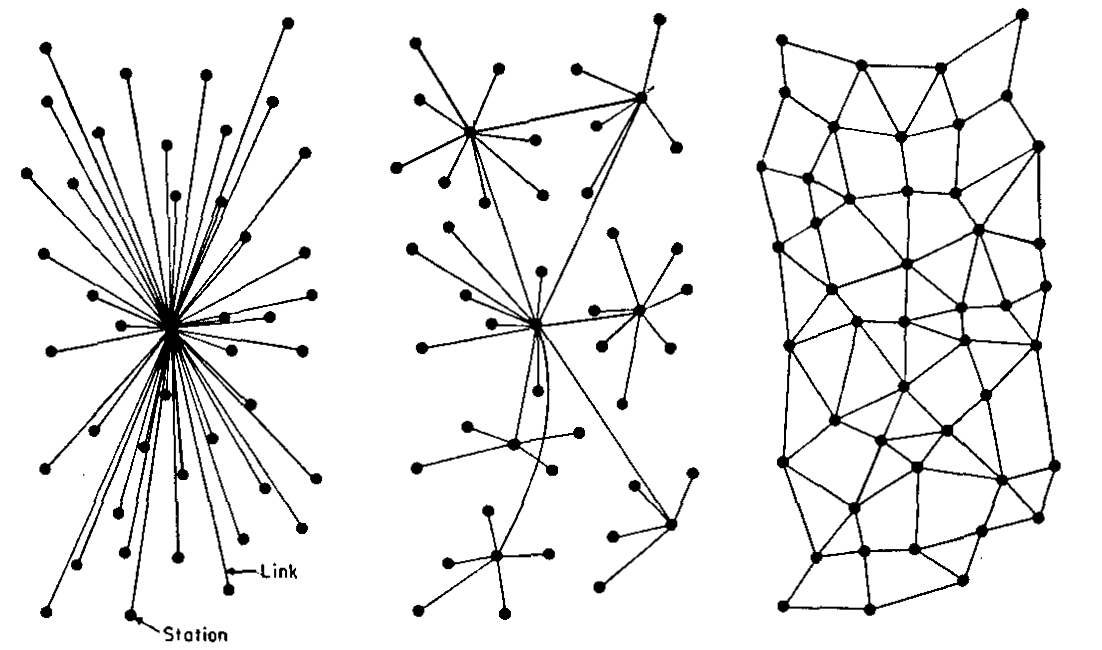
\includegraphics[trim=26cm 0cm 1cm 0cm, clip]{img/centralised-decentralised-distributed}
  }
  \caption[Caption for distributed-system]{
    Représentation d'une architecture distribuée \cite{1964-distributed-communications-networks-baran}.
    Ici, tout noeud du graphe correspond à un pair du système \ac{P2P}.}
  \label{fig:distributed-system}
\end{figure}

Récemment, la conception de systèmes collaboratifs \ac{P2P} a gagné en traction suite à \cite{localfirstsoftware2019}.
Dans cet article, les auteurs définissent un ensemble de propriétés qui correspondent à celles que nous avons établies précédemment, de la \autoref{def:collaborative-system} à la \autoref{def:censorship}.
En utilisant ces propriétés comme critères, les auteurs comparent les fonctionnalités et garanties offertes par les différents types d'applications, notamment les applications lourdes et les applications basées sur le cloud.

Le résultat de cette comparaison est le suivant : alors que les applications basées sur le cloud permettent de nouveaux usages, notamment la collaboration entre utilisateur-rices ou la synchronisation automatique entre appareils, elles retirent à leurs utilisateur-rices toute garantie de pérennité, confidentialité des données et souveraineté des données.
Ces dernières propriétés sont pourtant communément offertes par les applications lourdes.
La \autoref{fig:lfs-comparison-apps} détaille ce résultat.

\begin{figure}[!ht]
  \centering
  \resizebox{\columnwidth}{!}{
    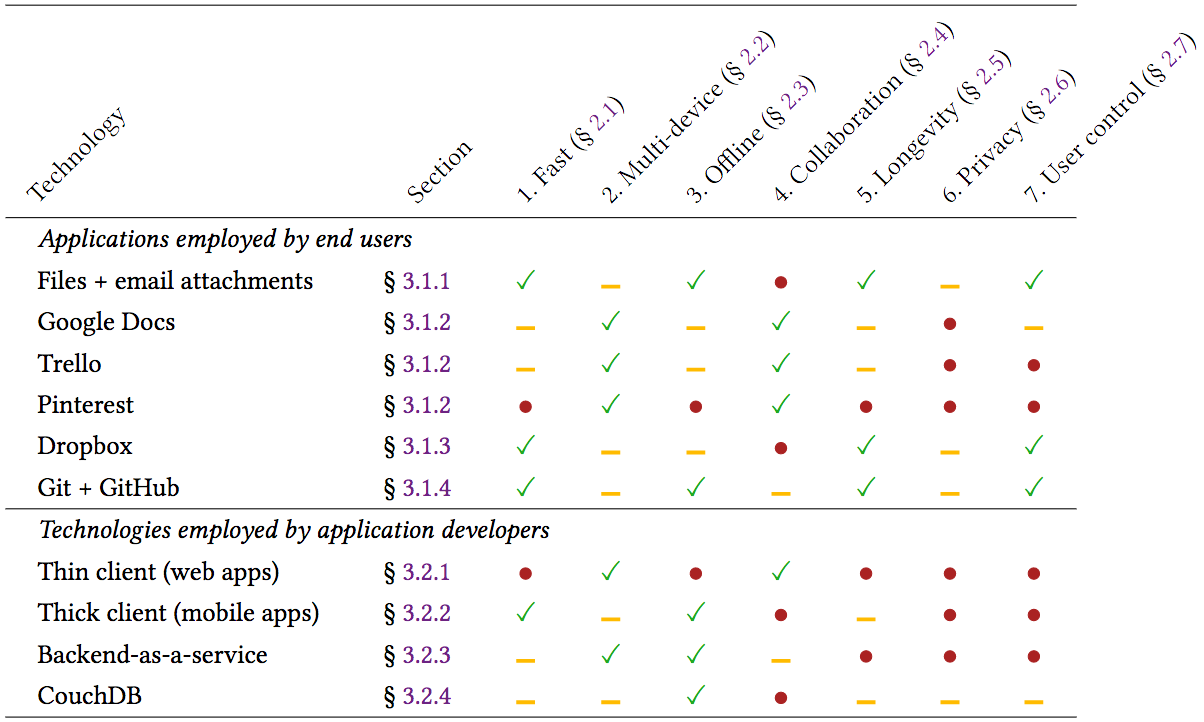
\includegraphics{img/lfs-comparison-apps}
  }
  \caption[Caption for lfs-comparison-apps]{
    Évaluation d'applications et de technologies vis-à-vis des 7 propriétés visées par les applications \aclp{LFS} \cite{localfirstsoftware2019}.
    {\color{lfsgreen} \checked}, {\color{lfsorange} \Flatsteel} et {\scriptsize \color{lfsred} \ding{108}} indiquent respectivement que l'application ou la technologie satisfait pleinement, partiellement ou aucunement le critère évalué.
  }
  \label{fig:lfs-comparison-apps}
\end{figure}

Malgré ce que ce résultat pourrait suggérer, les auteurs affirment que les nouveaux usages offerts par les applications basées sur le cloud ne sont pas antinomiques avec les propriétés de confidentialité, souveraineté, pérennité.

Ainsi, ils proposent un nouveau paradigme de conception d'applications collaboratives \ac{P2P}, nommées \acp{LFS}.
Ce paradigme vise à la conception d'applications offrant le meilleur des approches existantes, \ie des applications cochant l'intégralité des critères de la \autoref{fig:lfs-comparison-apps}.
Nous partageons cette vision.\\
% Ce type d'applications se démarque de ceux existants, \eg les applications basées sur le cloud, par la place centrale donnée aux utilisateur-rices et leurs propres appareils, les éventuels serveurs étant relegués qu'à de simples rôles de support.

Cependant, de nombreuses problématiques de recherche identifiées dans \cite{localfirstsoftware2019} sont encore non résolues et entravent la démocratisation des applications \acp{LFS}, notamment celles à large échelle.
Spécifiquement, les applications \acp{LFS} se doivent de répliquer les données entre les appareils pour permettre :
\begin{enumerate}
  \item Le fonctionnement en mode hors-ligne et le fonctionnement avec une faible latence.
  \item Le partage de contenu entre appareils d'un-e même utilisateur-rice.
  \item Le partage de contenu entre utilisateur-rices pour la collaboration.
\end{enumerate}

Toutefois, compte tenu des propriétés visées par les applications \acp{LFS}, plusieurs contraintes restreignent le choix des méthodes de réplication possibles.
Ainsi, pour permettre le fonctionnement en mode hors-ligne de l'application, \ie la consultation et la modification de contenu, les applications \acp{LFS} doivent relaxer la propriété de cohérence des données.
\begin{definition}[Cohérence]
  La cohérence d'un système indique sa capacité à présenter une vue uniforme de son état à chacun de ses utilisateur-rices à un moment donné.
\end{definition}

Les applications \acp{LFS} doivent donc adopter des méthodes de réplication dites optimistes \cite{2005-optimistic-replication-saito}.
Ces méthodes autorisent chaque noeud possédant une copie de la donnée à la consulter et à la modifier sans coordination au préalable avec les autres noeuds\footnote{Par opposition aux méthodes de réplication dites pessimistes, qui nécessitent une coordination préalable entre les noeuds avant toute modification de la donnée.}.
L'état des copies des noeuds peut donc diverger temporairement.
Un mécanisme de synchronisation permet ensuite aux noeuds de partager les modifications effectuées et de les intégrer de façon à converger à terme \cite{10.1145/224057.224070}, \ie obtenir à terme de nouveau des états équivalents.

Cependant, il convient de noter que les méthodes de réplication optimistes autorisent la génération en concurrence de modifications provoquant un conflit, \eg la modification et la suppression d'une même page dans un wiki.
Un mécanisme de résolution de conflits est alors nécessaire pour assurer la convergence à terme des noeuds.

De nouveau, le modèle du système des applications que nous visons, \ie des applications \acp{LFS} à large échelle, limitent les choix possibles concernant les mécanismes de résolution de conflits.
Notamment, ces applications ne disposent d'aucun contrôle sur le nombre de noeuds qui compose le système, \ie le nombre d'appareils utilisés par l'ensemble de leurs utilisateur-rices.
Ce nombre de noeuds peut donc croître de manière non-bornée.
Les mécanismes de résolution de conflits choisis devraient donc rester efficaces, de manière indépendante à l'évolution de ce paramètre.

De plus, les noeuds composant le système n'offrent aucune garantie sur leur stabilité.
Des noeuds peuvent donc rejoindre et participer au système, mais uniquement de manière éphèmère.
Ce phénonème est connu sous le nom de \emph{churn} \cite{understandingChurnP2PNetworks2006}.
Ainsi, de part l'absence de garantie sur le nombre de noeuds connectés de manière stable, les applications \acp{LFS} à large échelle ne peuvent pas utiliser des mécanismes de résolution de conflits reposant sur une coordination synchrone d'une proportion des noeuds du système, \ie sur des algorithmes de consensus \cite{1998-paxos-lamport, 2014-raft-ongaro}.

Ainsi, pour permettre la conception d'applications \acp{LFS} à large échelle, il convient de disposer de mécanismes de résolution de conflits pour l'ensemble des types de données avec une complexité algorithmique efficace peu importe le nombre de noeuds et ne nécessitant pas de coordination synchrone entre une proportion des noeuds du système.
